% -*- mode: latex; coding: latin-1-unix -*- %

\documentclass[a4paper,11pt]{article}



\usepackage[utf8]{inputenc} % pour les accents
\usepackage[T1]{fontenc}
\usepackage[francais]{babel}
\usepackage{fullpage}
\usepackage{color}
\usepackage{amsmath}
\usepackage{url} 
\usepackage{makeidx}
\usepackage{amsmath}
\usepackage{wasysym}
\usepackage{float}
\usepackage{graphicx}
\usepackage{a4wide}
\usepackage{multirow}
\usepackage{afterpage}
\usepackage{pst-all} % Pour pstricks
\usepackage{moreverb}

\definecolor{gray}{gray}{0.85}

\title{
  \normalsize{\begin{flushright} MASTER 2 - Semestre 2 - 2009 \end{flushright}}
  \vspace{15mm}
  \hrule height 1mm
  \vspace{5mm}
  \Huge{\emph{Projet de fin d'étude\\\textsl{AltaRica et les robots.}}}
  \vspace{5mm}\hrule height 1mm
  \vspace{1cm}
}

\author{
  J\'{e}r\'{e}my BOYER\\
  Dorian CRANSAC\\
  Jean S\'{e}bastien DUBERNET\\
  Fabien KUNTZ\\
  \vspace{2cm}
}

\date{}

\begin{document}
\begin{titlepage}
  \begin{figure}
    \vspace{1cm}
    \psset{unit=1in,linewidth=4pt} %paramtrage des units pour pstricks
    \rput(1,0){\includegraphics[width=4cm]{Bordeaux1}}
    \vspace{15mm}
  \end{figure}
\end{titlepage}

\maketitle

\vspace{4cm}
\begin{center}
Enseignant : Alain GRIFFAULT
\end{center}

\tableofcontents

\newpage
\begin{abstract}

Nous allons vous pr\'{e}senter dans ce rapport notre projet de fin d'\'{e}tude, qui consiste en l'application du cours de conceptions formelles sur la programmation de robots. Les robots en question sont les robots NXT de l'entreprise lego, sur lesquels nous utilisons le langage C. Ces robots sont capables de r\'{e}agir et m\^{e}me d'interagir avec leur environnement gr\^{a}ce \`{a} un ensemble de capteurs et de moteurs. Et nous allons utiliser le langage Altarica pour montrer que la mission que nous allons implémenter dans les robots est sure. Pour réaliser ce projet, nous avons procédés par étapes.\newline

Premièrement, nous avons du nous familiariser avec les robots NXT, les possibilités des différents capteurs, moteurs et constructions. Les possibilités niveau code ont aussi été éxaminées, tout ceci afin de savoir quel type de mission est réalisable. Puis nous avons décidés de cette mission.\newline

Deuxièmement, nous avons codés cette mission en langage C avec l'API NXC, et au fur et à mesure de la rédaction de cette mission, nous avons modélisés les noeuds Altarica correspondants aux différents capteurs, moteurs, au module bluetooth et au controlleur, pour obtenir au final une modélisation du robot maître et une modélisation du robot esclave, dans le contexte de la mission que nous avons choisi. \newline

Troisièmement, il s'agit de prouver grâce à une spécification $Acheck$ pour chaque noeud Altarica que ce dernier est sur et ne provoque pas de comportements non désirés. \newline

Enfin, quatrièmement, nous avons fait une analogie entre nos noeuds Altarica et le code C de nos robots, afin de créer une piste vers une pseudo génération automatique de code faisant fonctionner les robots à partir des modélisations Altarica.\newline


\end{abstract}





 \begin{frame}
  \frametitle{Mission}
  
  \begin{block}{Matériel}
   \begin{itemize}
    \item Eléments de base LEGO
	  \uncover<2->{
    \item Capteurs}
	  \uncover<3->{
    \item Moteurs}
	  \uncover<4->{
    \item Damier blanc/gris + feuilles noires pour les obstacles}
   \end{itemize}
  \end{block}

  \uncover<5->{
  \begin{block}{Objectif}
   \begin{itemize}
    \item Progression du maître dans le "labyrinthe" (succession de comportements de base)
	  \uncover<6->{
    \item Communication des ordres à l'esclave}
	  \uncover<7->{
    \item Atteinte de la sortie}
   \end{itemize}
  \end{block}
  }

 \end{frame}

 \begin{frame}
  \frametitle{Le Damier - justification}
 \center
  \includegraphics[height=5cm]{damier.eps}
  \end{frame}

\section{R\'{e}duction API NXC}
Pour la r\'{e}alisation du  projet nous utiliserons 4 cat\'{e}gories de fonction : celles relatives aux moteurs, aux capteurs , à la connexion Bluetooth et \'{e}ventuellement d'autres fonctions permettant la coh\'{e}sion de l'ensemble.

\subsection{Les moteurs }
\begin{verbatim}
	OnFwd("port","power"); //permet de mettre en marche "avant" un moteur du robot 
	OnRev("port","power"); //sens inverse
	RotateMotor("port","speed","degrees"); //
	RotateMotorEx("port","speed","degrees","turnpct","sync","stop"); 
\end{verbatim}

\subsection{Les capteurs }

\subsubsection{Type et mode des capteurs}
\begin{verbatim}
	SetSensorLight("port"); //Lie le capteur de lumière à un "port"
	SetSensorSound("port"); //Lie le capteur ultrason à un "port"
	SetSensorMode("port","const mode"); //Configure le mode du capteur associé au "port"
	SetInput("port","const field","value"); //Configure le type du capteur associé au "port"
	SetSensorLowspeed("port"); //Configure le capteur en mode I2C
	ClearSensor("port"); //Efface la valeur d'un capteur associé à un "port"

\end{verbatim}

\subsubsection{Information des capteurs}
\begin{verbatim}
	Sensor("n"); //retourne la valeur d'un capteur
	SensorUS("n"); //retourne la valeur du capteur ultrason

\end{verbatim}

\subsection{La connexion Bluetooth }
\begin{verbatim}
	BluetoothStatues("NUMBER"); //Vérifie la connexion
	RemoteStartProgram("connection", "filename");
	RemoteStopProgram("connection");

\end{verbatim}

\subsection{Autres fonctions }
\begin{verbatim}
	Wait("time"); //Temps donné à l'exécution d'une action
	off("port"); //Stop le moteur associé au "port"
	Acquire("mutex"); 
	Release("mutex"); 
	Precedes("task1","task2","taskn"); //Permet l'exécution de taches simultané

\end{verbatim}

\subsection{Les variables }
\begin{verbatim}
	OUT_A; //port A
	OUT_AC; //port AC
	IN_1; //Input 1
	IN_2; //Input 2

\end{verbatim}
 \section{AltaRica}

  \subsection{Architecture}
  \begin{figure}[!ht]
   \begin{center}
    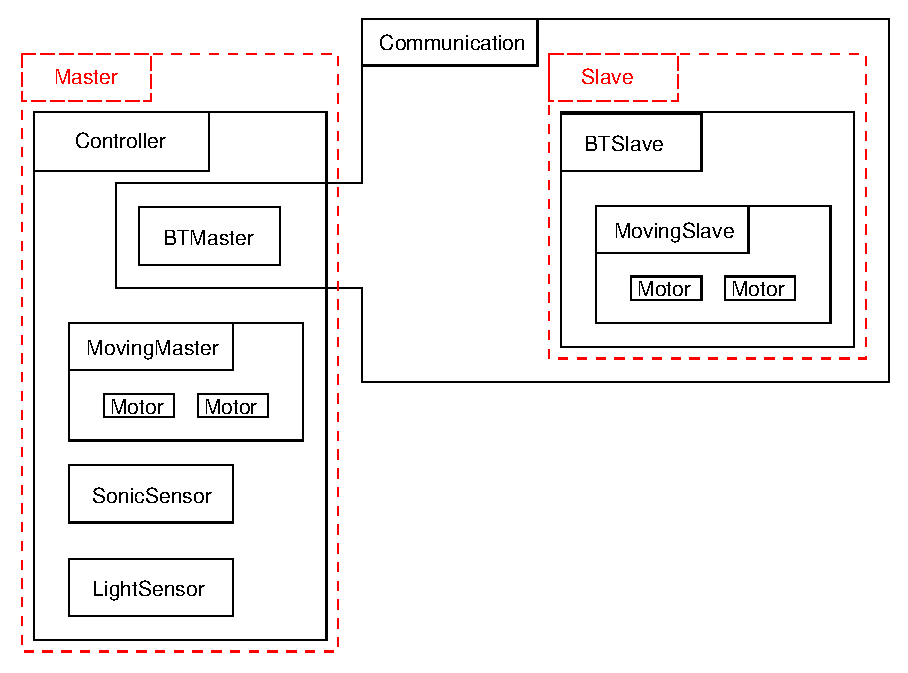
\includegraphics{ARmodel.eps}
    \caption{Architecture AltaRica}
   \end{center}
  \end{figure}

  \subsection{Les capteurs et moteurs}
    
   \subsubsection{Le n\oe{}ud LightSensor}

    \paragraph{\underline{Description\\}}
    Ce noeud correspond au capteur de lumière, et possède une variable
    d'état nommée $color$ qui   peux prendre trois valeurs différentes,
    correspondants au trois couleurs de case que nous allons utiliser:
    Noir, gris et blanc. Cette variable d'état n'est présente que pour
    pouvoir modéliser des événements, qui seront déclenché par les
    différentes valeurs de la variable de flux $value$. L'action du
    senseur de lumière est donc véritablement représentée par cette
    variable de flux, puisque les valeurs lues par le senseur sont
    "incontrôlables".

    \paragraph{\underline{Le source Altarica\\}}
    \verbatiminput{../src/altarica/alt/LightSensor.alt}
   
    \paragraph{\underline{La spécification\\}}
    \verbatiminput{../src/altarica/acheck/LightSensor.acheck}

    \paragraph{\underline{La sémantique\\}}
    \begin{figure}[!ht]
     \begin{center}
      \includegraphics{../src/altarica/LightSensor.eps}
      \caption{LightSensor}
     \end{center}
    \end{figure}

    \paragraph{\underline{Les résultats\\}}
    \verbatiminput{../src/altarica/LightSensor.prop}
    \verbatiminput{../src/altarica/LightSensor.res}
   
   \subsubsection{Le n\oe{}ud UltraSonicSensor}
   
    \paragraph{\underline{Description\\}}
    De la même manière que le noeud LightSensor, UltraSonicSensor
    comporte une variable d'état "behind" qui servira à pouvoir
    déclencher les deux évènements $readValue$. Le principe du capteur
    est que soit il y a un objet capté, soit il n'y en a pas, sans
    distinction véritable de distance. Et comme pour LightSensor, c'est
    la variable de flux $d$ qui déclenche ces évènements.

    \paragraph{\underline{Le source Altarica\\}}
    \verbatiminput{../src/altarica/alt/UltraSonicSensor.alt}
    
    \paragraph{\underline{La spécification\\}}
    \verbatiminput{../src/altarica/acheck/UltraSonicSensor.acheck}
    
    \paragraph{\underline{La sémantique\\}}
    \begin{figure}[!ht]
     \begin{center}
      \includegraphics{../src/altarica/UltraSonicSensor.eps}
      \caption{UltraSonicSensor}
     \end{center}
    \end{figure}

    \paragraph{\underline{Les résultats\\}}
    \verbatiminput{../src/altarica/UltraSonicSensor.prop}
    \verbatiminput{../src/altarica/UltraSonicSensor.res}
   
   \subsubsection{Le n\oe{}ud Motor}
  
    \paragraph{\underline{Description\\}}
    Les moteurs sont modélisés de façon à avoir seulement trois vitesses
    possible: Avancer, stopper, reculer.

    \paragraph{\underline{Le source Altarica\\}}
    \verbatiminput{../src/altarica/alt/Motor.alt}
    
    \paragraph{\underline{La spécification\\}}
    \verbatiminput{../src/altarica/acheck/Motor.acheck}
    
    \paragraph{\underline{La sémantique\\}}
    \begin{figure}[!ht]
     \begin{center}
      \includegraphics{../src/altarica/Motor.eps}
      \caption{Motor}
     \end{center}
    \end{figure}

    \paragraph{\underline{Les résultats\\}}
    \verbatiminput{../src/altarica/Motor.prop}
    \verbatiminput{../src/altarica/Motor.res}
   
  \subsection{Les déplacements, n\oe{uds Moving}}

    \paragraph{\underline{Description\\}}
    Les n\oe{}uds Moving sont là pour faire la synchronisation entre les deux moteurs
    munis de roues d'un robot. Il y a cinq ordres possible: Avancer,
    s'arrêter, reculer, à droite et à gauche. Il faut savoir que les
    rotations à droite et à gauche du robot sont tout le temps de 90
    degrés.

    \paragraph{\underline{Les sources Altarica\\}}
    \verbatiminput{../src/altarica/alt/MovingMaster.alt}
    \verbatiminput{../src/altarica/alt/MovingSlave.alt}
    
    \paragraph{\underline{Les spécifications\\}}
    \verbatiminput{../src/altarica/acheck/MovingMaster.acheck}
    \verbatiminput{../src/altarica/acheck/MovingSlave.acheck}
    
    \paragraph{\underline{La sémantique\\}}
    \begin{figure}[!ht]
     \begin{center}
      \includegraphics[width=16cm]{../src/altarica/MovingMaster.eps}
      \caption{MovingMaster}
     \end{center}
    \end{figure}

    \begin{figure}[!ht]
     \begin{center}
      \includegraphics[width=16cm]{../src/altarica/MovingSlave.eps}
      \caption{MovingSlave}
     \end{center}
    \end{figure}

    \paragraph{\underline{Les résultats\\}}
    \verbatiminput{../src/altarica/MovingMaster.prop}
    \verbatiminput{../src/altarica/MovingMaster.res}
    ~\newline
    \verbatiminput{../src/altarica/MovingSlave.prop}
    \verbatiminput{../src/altarica/MovingSlave.res}
    
  \subsection{La communication}
    
   \subsubsection{Les n\oe{}uds BTMaster, BTSlave et MasterSlave}
    
    \paragraph{\underline{Description\\}}
    La communication bluetooth entre les deux robots est de type
    maitre/esclave, le maitre envoie simplement des ordres à executer à
    l'esclave. Le noeud BTMaster qui sera pour le robot maitre comporte
    donc simplement les cinq même ordres que le noeud moving. BTSlave
    sera lui pour le robot esclave, et inclus un sous noeud de type
    Moving, afin de pouvoir synchroniser les cinq ordres possibles à un
    agissement concret de ce noeud Moving. Enfin, le noeud MasterSlave se
    chargera de faire la synchronisation entre les ordres des noeuds
    BTMaster et BTSlave.

    \paragraph{\underline{Les sources Altarica\\}}
    \verbatiminput{../src/altarica/alt/BTMaster.alt}
    \verbatiminput{../src/altarica/alt/BTSlave.alt}
    \verbatiminput{../src/altarica/alt/BTMasterSlave.alt}
    
    \paragraph{\underline{Les spécifications\\}}
    \verbatiminput{../src/altarica/acheck/BTMaster.acheck}
    \verbatiminput{../src/altarica/acheck/BTSlave.acheck}
    \verbatiminput{../src/altarica/acheck/BTMasterSlave.acheck}

    \paragraph{\underline{La sémantique}}
    \begin{figure}[!ht]
     \begin{center}
      \includegraphics[width=16cm]{../src/altarica/BTMaster.eps}
      \caption{BTMaster}
     \end{center}
    \end{figure}
    \begin{figure}[!ht]
     \begin{center}
      \includegraphics[width=16cm]{../src/altarica/BTSlave.eps}
      \caption{BTSlave}
     \end{center}
    \end{figure}
    \begin{figure}[!ht]
     \begin{center}
      \includegraphics[width=16cm]{../src/altarica/BTMasterSlave.eps}
      \caption{BTMasterSlave}
     \end{center}
    \end{figure}
   
  \subsection{Le n\oe{}ud Controller}
   
    \paragraph{\underline{Le source Altarica\\}}
    \verbatiminput{../src/altarica/alt/Controller.alt}
    
    \paragraph{\underline{La spécification\\}}
    \verbatiminput{../src/altarica/acheck/Controller.acheck}
    
    \paragraph{\underline{La sémantique\\}}
    \begin{figure}[!ht]
     \begin{center}
      
\includegraphics[width=16cm]{../src/altarica/Controller.eps}
      \caption{Controller}
     \end{center}
    \end{figure}

    \paragraph{\underline{Les résultats\\}}
    \verbatiminput{../src/altarica/Controller.prop}
    \verbatiminput{../src/altarica/Controller.res}

\section{Génération de code à partir des noeuds altarica élémentaires.}

Etant donné que notre modèle altarica représente les comportements des éléments du système, nous allons ici faire le lien entre chaque comportement adopté par une entité et des portions de code implémentant ces comportements.

\subsection{Motor}

\begin{verbatim}
event
    	back		OnFwd(Out_X, Y); pour le moteur X, et Y choisi arbitrairement entre 1 et 100.
    	stop		OnFwd(Out_X, 0);
    	forward	OnRev(Out_X, Y); pour le moteur X, et Y choisi arbitrairement entre 1 et 100.

\end{verbatim}

La conjonction des évenements des 2 moteurs permettent de déplacer le robot de manière cohérente. Ceci correspond au noeud Moving.

\subsection{Moving}

\begin{verbatim}
event
	stop	OnFwd(Out_AC, 0);
	left	OnFwd(Out_C, 20); et OnRev(Out_A, 20); ou bien RotateMotorEx(OUT_AC, 40, 180, -100, true, true); (plus simple)
	forward	OnFwd(Out_AC, 40);
	right		OnFwd(Out_A, 20); et OnRev(Out_C, 20); ou bien RotateMotorEx(OUT_AC, 40, 180, 100, true, true); (plus simple)
	halfturn	RotateMotorEx(OUT_AC, 40, 360, 100, true, true);
\end{verbatim}

\subsection{LightSensor}

\begin{verbatim}
flow
    value : [0,2];	value = SensorUs(3); 3 étant dans notre cas le numéro du port sur lequel est branché le capteur lumineux.
\end{verbatim}

\subsection{UltraSonicSensor}

\begin{verbatim}
flow
    d : bool;	value = SensorUs(4); 4 étant dans notre cas le numéro du port sur lequel est branché le capteur ultrason.

\end{verbatim}

\subsection{BlueTooth}
% -*- mode: latex; coding: latin-1-unix -*- %
\section{Bilan}

\subsection{Difficultées rencontrées}

\subsubsection{Problématique du damier}

Nous avions initialement prévu que la mission se déroulerait dans un environnement ou le sol serait homogène (exemple: tout blanc). Cependant, un problème de décision est survenu. Il était impossible de différencier la présence de l'absence d'un chemin à gauche ou à droite lors de la rencontre d'un obstacle. Etant donné que le robot reste sur la même case lors de sa rotation, il aurait fallu décider d'une distance ou durée avant la rencontre potentielle d'un nouvel obstacle sur le nouveau chemin, ce qui va à l'encontre  de l'objectif de réactivité et généricité du comportement du robot. Pour éviter de temporiser cette action, nous avons décidé d'utiliser un damier gris et blanc, permettant de décider au premier changement de case sur le nouveau chemin si ce chemin est effectivement utilisable ou si la solution était la direction opposée (rencontre immédiate d'une nouvelle case noire).

\subsubsection{Problématique de seuil intermédiaire du capteur lumineux}

Lors du passage du capteur entre les 2 seuils extrêmes (case blanche à case noire ou case noire à case blanche), le capteur détecte un seuil intermédiaire gris pendant un bref instant, causant un bug dans la prise de décision. Nous avons du mettre en place un procédé de correction de la detection qui renouvelle la lecture du capteur après un très bref instant et change la valeur obtenue si elle est différente de la dernière lecture. Cette temporisation était incontournable.

\subsection{Conclusion}

\end{document}
